\section{Mathematics and Programming}
\begin{frame}{Kinematic Model}{Aleksandra Zasadni}
\begin{columns}
\column{0.4\textwidth}
    \begin{itemize}
        \item Mathematical Model 
        \begin{itemize}
            \item Behaviour
            \item Tasks
        \end{itemize}
        \item Kinematic model
    \end{itemize}    
\column{0.6\textwidth}
\centering{
\includegraphics[scale=0.17]{graphics/andrej/kuka}}

\tiny{(kuka.com)}
\end{columns}
\end{frame}

\begin{frame}{Kinematic Model}{Forward Kinematics}
\begin{columns}
\column{0.5\textwidth}
\begin{itemize}
    \item End-effector
    \item Joint variables
    \item Rigid transformation
    \item Separate rigid transform
    \item Denavit-Hartenberg
    \begin{itemize}
        \item Joint matrices
        \item Link matrices
        \item Standardised
    \end{itemize}
\end{itemize}
\column{0.5\textwidth}
\centering{
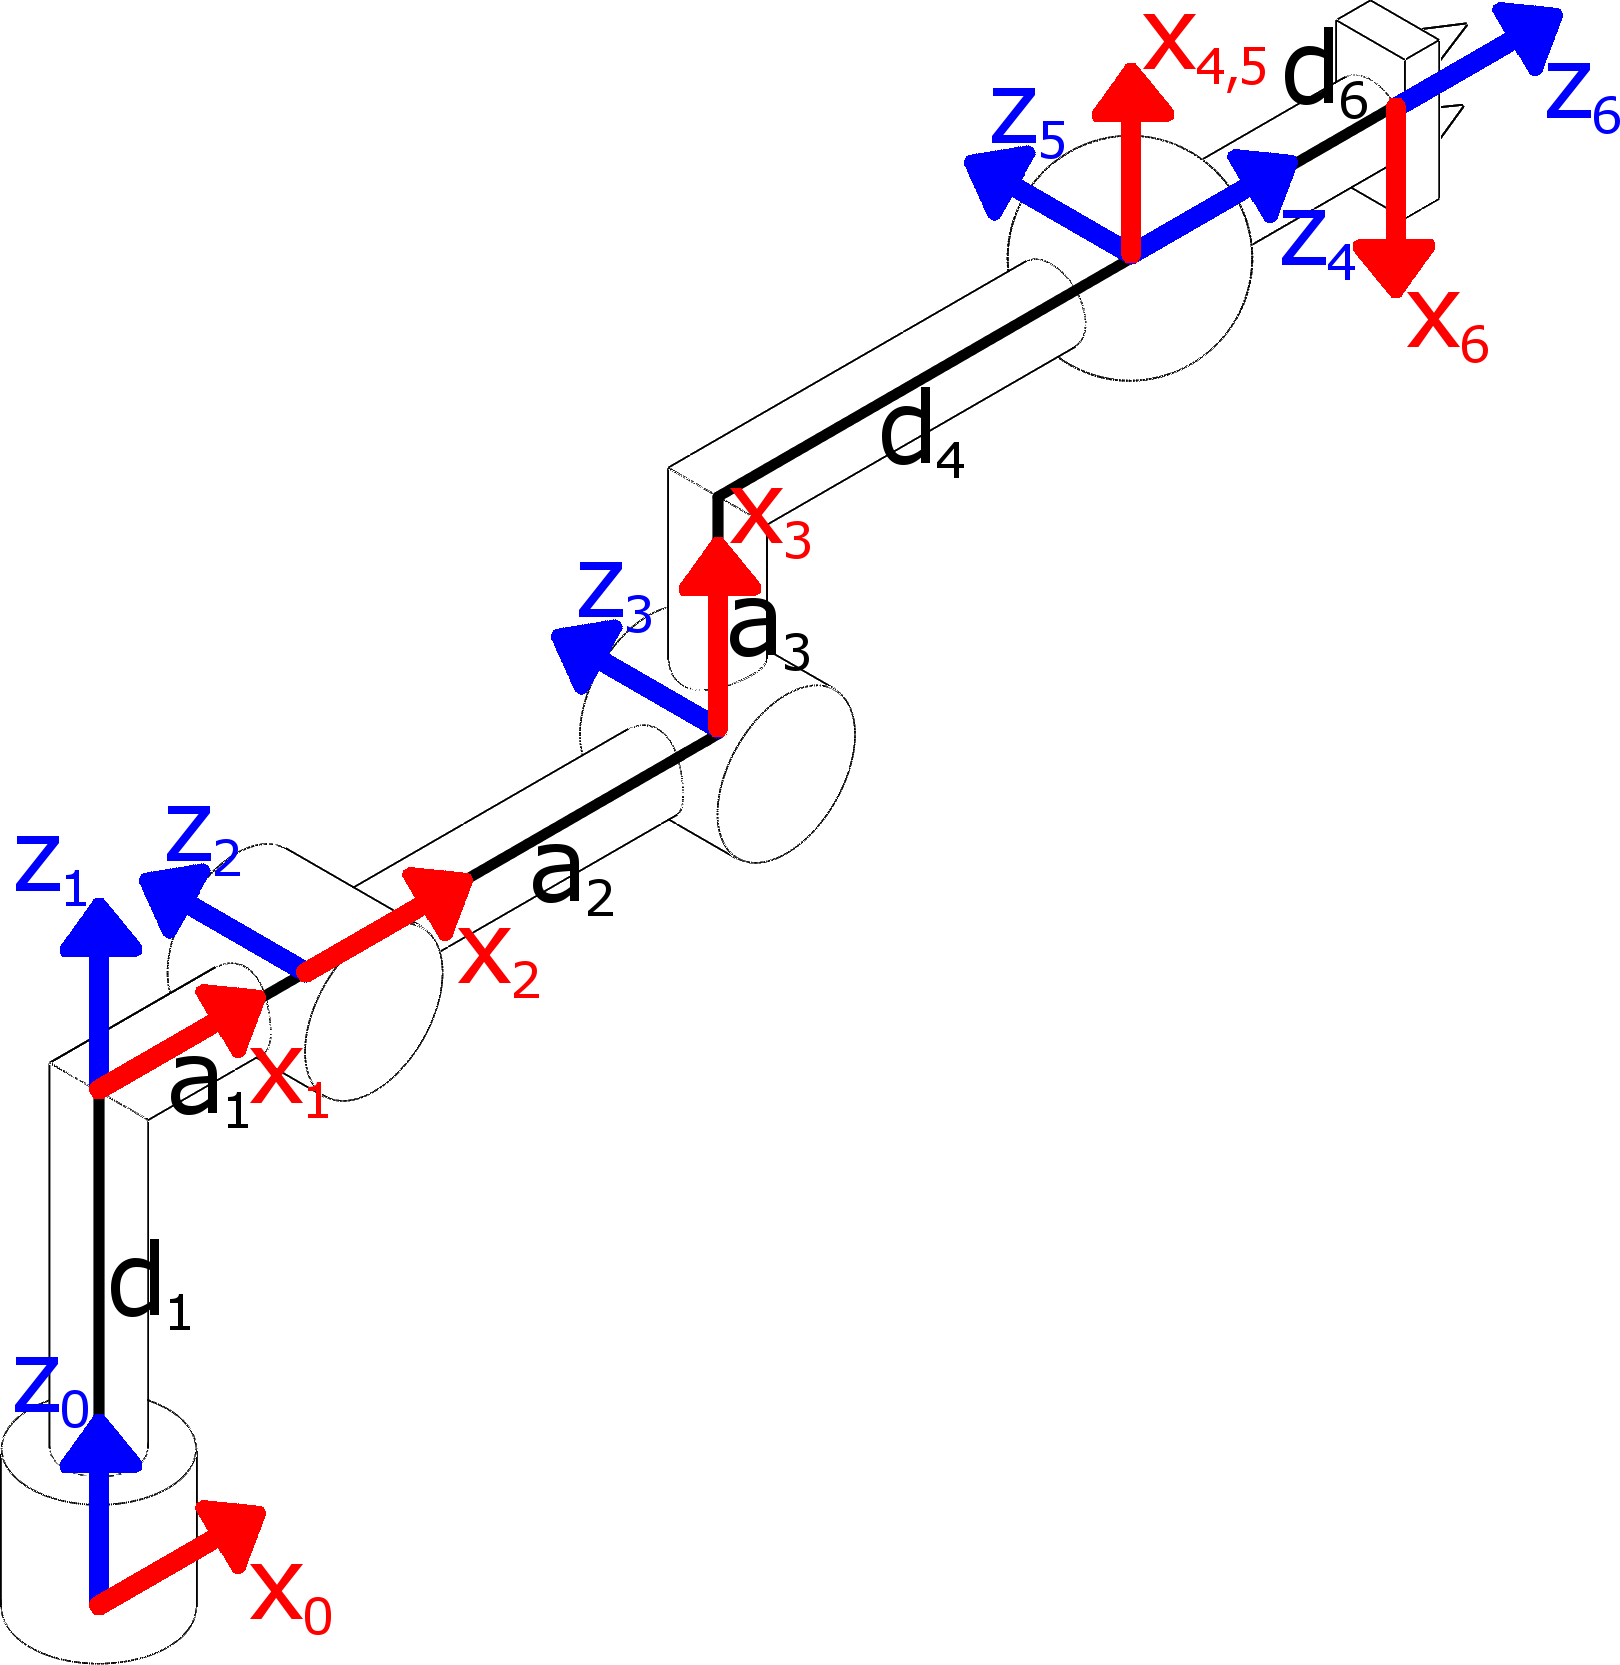
\includegraphics[scale=0.38]{graphics/alex/dh_param.png}}
\end{columns}
\end{frame}


\begin{frame}{Kinematic Model}{Inverse Kinematics}
\begin{itemize}
    \item Joint variables
    \item Position and orientation of end-effector
    \item Application
    \begin{itemize}
        \item Cartesian coordinates
    \end{itemize}
    \item Approach 
    \item Configurations
    \item Solutions
\end{itemize}
\end{frame}

\begin{frame}{Kinematic Model}{Trajectory Planning}
\begin{itemize}
    \item Joint space trajectory
    \item Cartesian space trajectory
    \item Advantages and disadvantages
\end{itemize}
\end{frame}

\begin{frame}{Programming}{Off-line and On-line}
\begin{columns}
\column{0.4\textwidth}
\begin{itemize}
    \item Off-line vs On-line
    \begin{itemize}
        \item Advantages
        \item Disadvantages
    \end{itemize}
    \item \textit{UR5}
    \begin{itemize}
        \item \textit{PolyScope}
        \item \textit{URScript}
    \end{itemize}
\end{itemize}
\column{0.6\textwidth}
\centering{
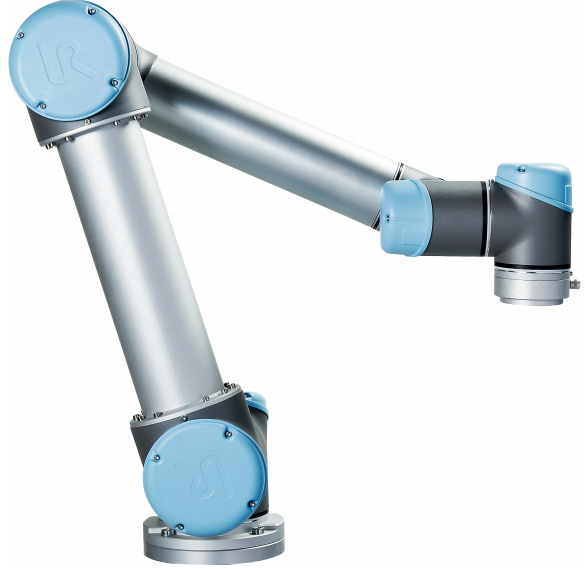
\includegraphics[scale=0.27]{graphics/alex/ur5_design.png}}
\end{columns}
\end{frame}

\begin{frame}{Programming}{RobotStudio}
\begin{columns}
\column{0.5\textwidth}
\begin{itemize}
    \item CAD model
    \item Geometries
    \item Waypoints
    \item Orientation representation
    \item Conversion script
\end{itemize}

\column{0.5\textwidth}
\centering{
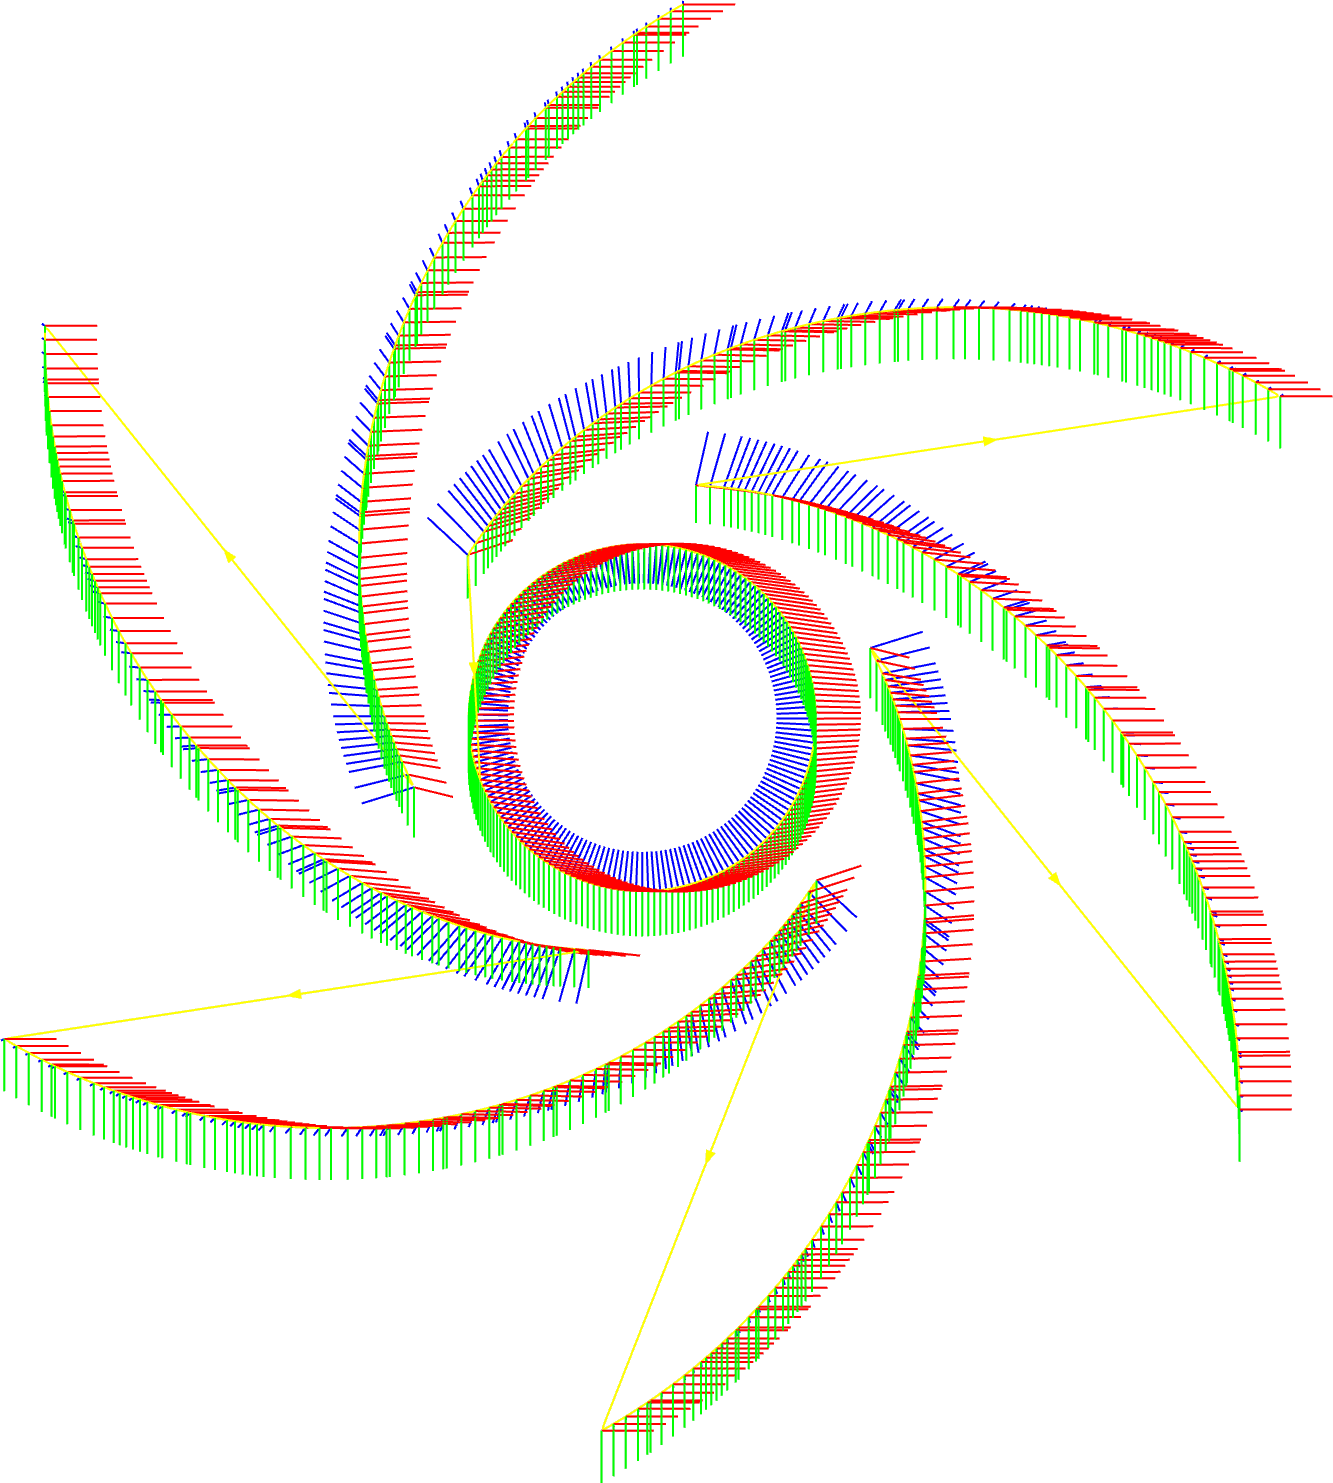
\includegraphics[scale=0.099]{graphics/alex/trajectory_1.png}}
\end{columns}
\end{frame}